#programming
#programming/vim
# Purpose of this File
(2021-04-08 D:-GitHub-AQ-Ref-Journals-Ipynb)
Track my edits in vs code (copy over links and problems between .ipynb notebooks)
\section{Links}
[b]{chrome://bookmarks/}
[codecademy]{https://www.codecademy.com/learn}
[programming Google Photos]{https://photos.google.com/share/AF1QipOo3gv-kAJt7s0MGQBohEWMuOdEfNcYdcnQ6f45SavHoEWIxQ0yqbjS8oxlZZhvYQ?key=VUl3NkxkQ2ZuNDJiZ3Zmc0d1M3JzVXhsd2pTTjRB}
[keep]{https://keep.google.com}{Keep Matlab} ToDos \& Questions

\href{https://code.visualstudio.com/docs/getstarted/keybindings\#_editorwindow-management}{vs
code shortc{[}link text{]}(https://)uts}

\href{https://vim.rtorr.com/}{vim keyboard shortcuts}

\href{https://github.com/VSCodeVim/Vim}{vim readme}

\begin{verbatim}
I installed the extension learn vim. I can work thru the lessons by doing 
ctrl+shft+p then executing the command learn vim
\end{verbatim}
# Problems
#programming
\section{Problems}\label{problems}
## Polaroid
- [ ] Clean up this file using Neovim
    - The file was imported from an .ipynb file into .tex
    - While I am at Triumph I don't have access to a Vim editor other than Overleaf, but the "Visual Editor" in Overleaf is passable.
    - [ ] Programmatically delete whitespace /r carriages :%s...
    - [ ] Open a duplicate vertical window then rearrange my headings to be chronological.
## Setup
- IDK how to use "git bash" I deleted the replace shortcut for files,
  and made replace ctrl+shift+
A backup of my file is at **\href{https://drive.google.com/file/d/1zdhAzUpru31W0oSY7ZKPXnwiqQ31veED/view?usp=sharing}{settings.json}**
# 2023-06-07_1400
#programming
\section{Good Luck Babe}
- I copy pasted the first lines of "Introductory Programming"
    - [Sagecell PREP tutorials]{https://doc.sagemath.org/html/en/prep/index.html}
- Sage as a programming language has similar syntax to Python bc it was built on Python 3.
- I could still do Python 2 on codeacademy. I know that in Python 3 tabs can no longer be spaces, and there is not a print function that doesn't use ().
- [ ] Write a basic function on [Sagecell one off python]{https://sagecell.sagemath.org/}
# 2022-09-14_1333
#programming
- VS Code
  - If I do :reg \[:_reg_isters\], then I can see what's where
    - (my bkm **vim torr** also explains vim registers)
    - save to the clipboard with "+\[plus \]+y+\[movement \]
    - When I delete or yank something, it goes into the default numbered registers \[1,2,3\]
    - I access a register by first typing "
      - " Unnamed register last delete or yank
      - 0 Last yank
      - 1.. Numbered registers
      - \- Last small (less than a line) delete
      - \* Clipboard contents (X11 primary)
      - \+ Clipboard contents (X11 clipboard) (not shown, but still works)
      - . last _i_nserted text
      - \# Name of the first _folder_ that's open in VS Code
      - % file path ex: d:\\GitHub\\AQ-Ref-Journal...
      - / Last forward search
      - : Last command line
      - \= Expression register
      - _ **?** Black hole register
  - Clipboard
        - I changed the following settings
\begin{figure}
    \centering
    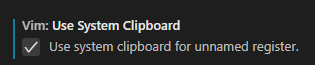
\includegraphics[width=0.5\linewidth]{vs code setting system clipboard.png}
    \caption{vs code setting system clipboard}
\end{figure}
       - for multicursor in VS Code, hold alt
# 2022-04-03_1334 Python

**The difference between a notebook and a file for calculating variables**

Ethan explained to me the difference between a notebook and a file.

- A python file can be ran in vs code (f5), and print out to the commandline. However, the variable states won't be saved unless I have made a break point (left click on a .py)
\begin{figure}
    \centering
    \includegraphics[width=0.5\linewidth]{VS Code Local variables in ipynb.png}
    \caption{VS Code Local variables in ipynb}
\end{figure}
- A jupyter notebook (.ipynb)
\begin{figure}
    \centering
    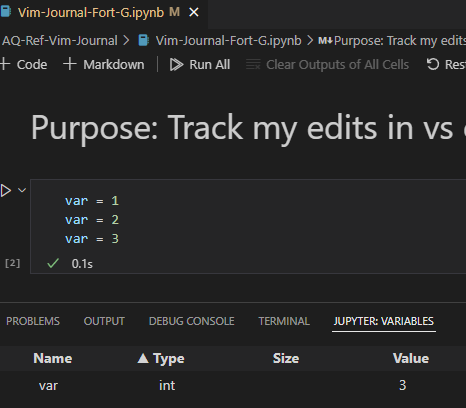
\includegraphics[width=0.5\linewidth]{VS Code Local variables in Jupyter section.png}
    \caption{VS Code Local variables in Jupyter section}
\end{figure}

# 2021-09-13_1234
#programming/github
I can open powershell in vs code by clicking Terminal\textgreater new\textgreater powershell\textgreater open in editor. 

% I installed git bash locally. It is in my start menu, and IDK how to use 
% it. The bottom left of my vs code screen shows that

I do remember how to use the gui Desktop gitHUB app though. I made a new
repo for tests called September-2021-Scratch. It is in:
C:\textbackslash Users\textbackslash dashf\textbackslash AndroidStudioProjects\textbackslash Free\_Code\_Tourism\textbackslash September-2021-Scratch

The github app lets me open my github files in vs code and windows
explorer directly

Whenever I install new programs, they don't take effect in powershell
until I restart powershell

I just us .md files for reading LaTeX in VS Code.

# 2021-09-05_1234
#programming/python
To run python code, if copying the terminal like google photos doesn't
work, then I can just press "ctrl + enter"

\begin{figure}
    \centering
    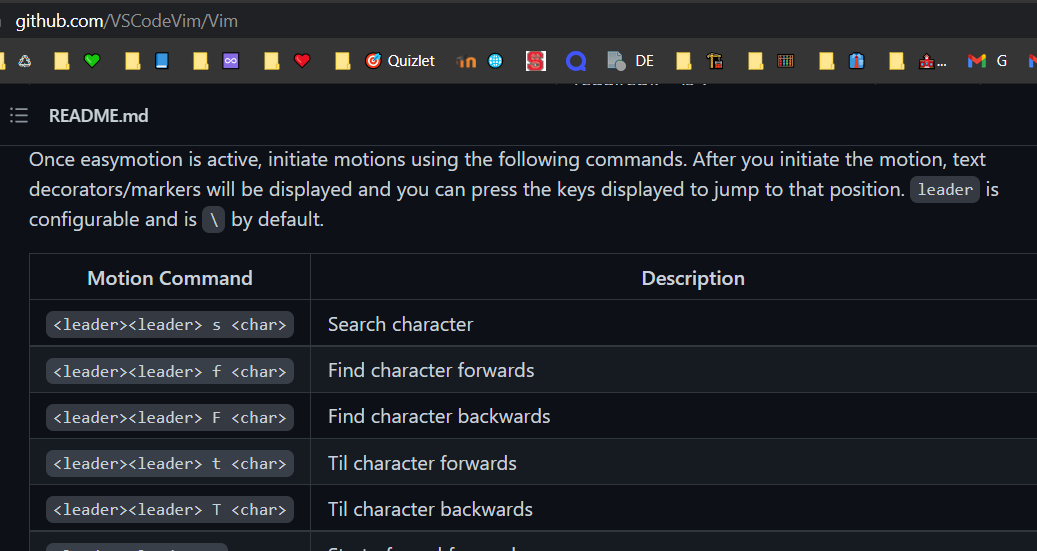
\includegraphics[width=1\linewidth]{easymotion.png}
    \caption{Vim Easymotion}
\end{figure}

- I played around with the
file\textgreater preferences\textgreater keyboard shortcuts, but i
couldnt get "add comment" to work (I think vim was interfearing)
Instead, to add a multiline comment, I will resort to surrounding the
block of code with '''
# 2021-04-07_1234
#programming
%%%%%%%%%%%%%%%%%%%%%%%%%%%%%%%%%%%%%
--------todo----------

- [ ] I need to backup my matlab files in github
  
- [ ] I need to make another overleaf project for my matlab notes
  
- [ ] I need to make a .sty in overleaf that works for notetaking

- [ ] I get 500 mb free storage in zotero. I need to set it up to manage bibliographies instead of using citation machine

- [ ] If the outline doesn't work, I could break up the sections at the top of this
journal into different files

--------notes---------

- I want these journals to be searchable for when I need to find how I have done something in the past

- [ ] read https://docs.github.com/en/get-started/quickstart/github-flow
  - in vs code, after I press ctrl+shift+P I can use non-vim hotekeys
%%%%%%%%%%%%%%%%%%%%%%%%%%%%%%%%%%%%%

# 2021-03-27_1234
#programming
\begin{itemize}
\tightlist
\item
  add to vs code: I think that typing shft+/ (questionmark) results in a
  universal search, but I don't know how to advance
\end{itemize}

-I deleted the replace shortcut for files, and made replace ctrl+shift+h

-\textbf{I can save how I have my files open in VS Code by going
file\textgreater save\textgreater workspace}

-I can use vim as a text editor too. This is my setup for sts' pdf on
the left, and my md file on the right. STS stands for science and technology at NCSU.

\begin{figure}
    \centering
    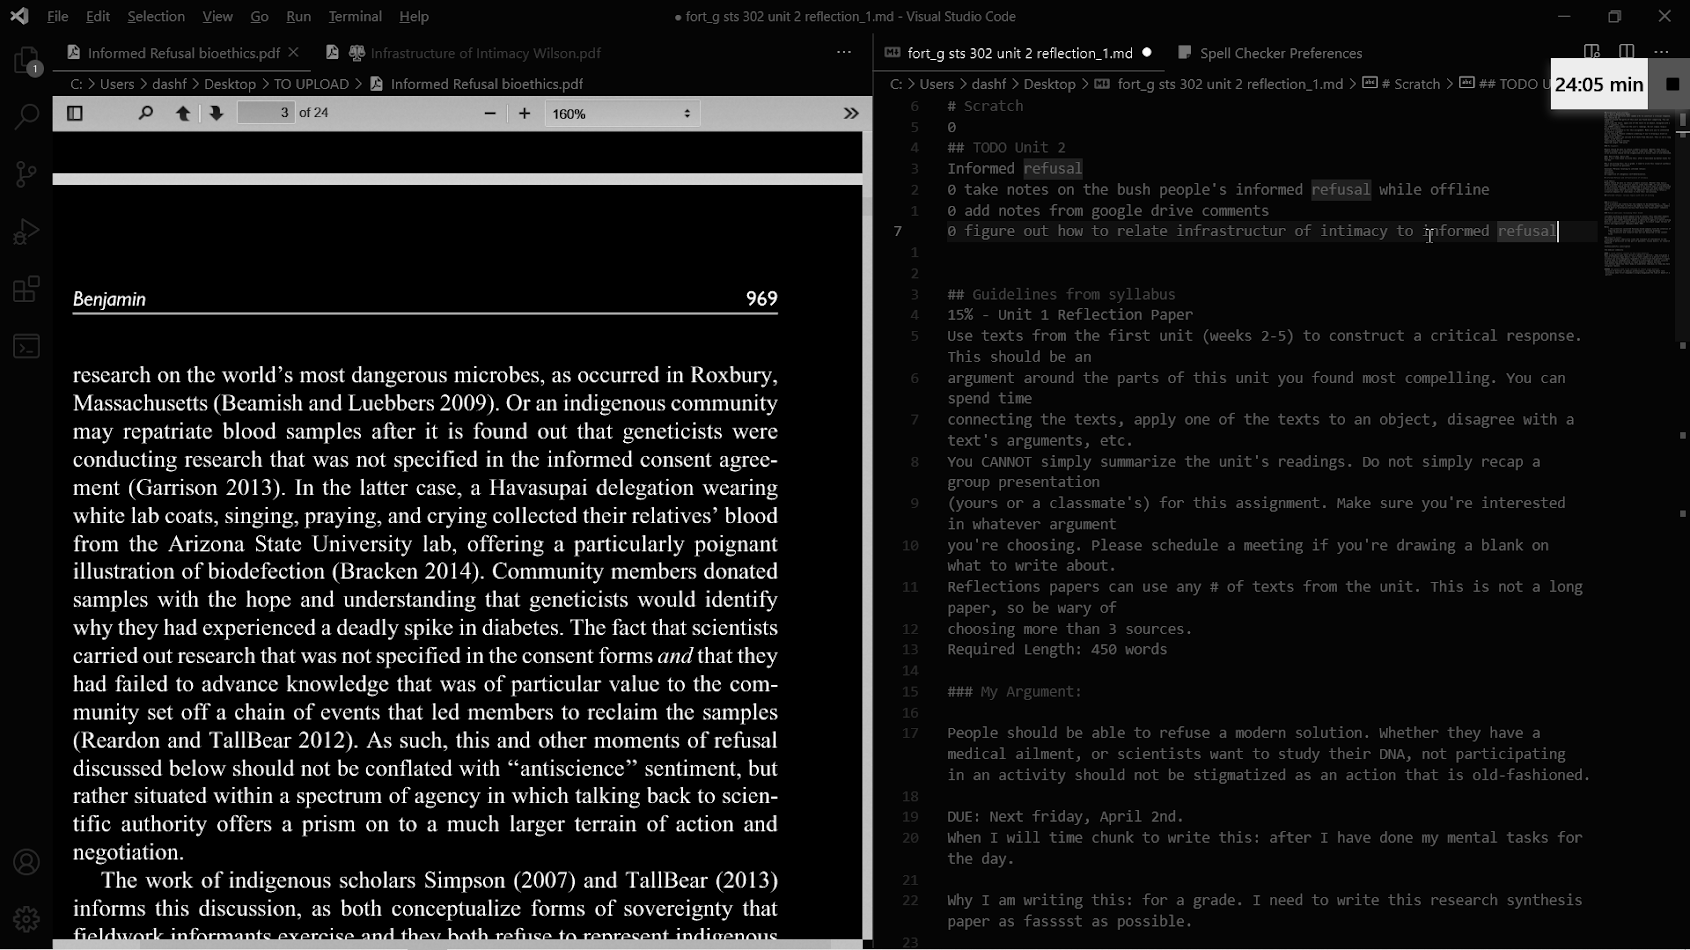
\includegraphics[width=1\linewidth]{vs code scrnsht.png}
    \caption{example pdf and markdown file in vs code}
\end{figure}
# 2021-03-15_1234
#programming
- I am still trying to figure out what is the best way for me to work with
a reference I didn't use the colab I made, Instead, I had: - a doc
called "outline", and the files for my project all on the right of my
screen pinned in VS code, - then I had the pdf of the assignment on the
left. - \% I just took notes in comments

- [ ] I deleted the replace shortcut for files, and made replace ctrl+shift+
I followed the youtube video
\url{https://www.youtube.com/watch?v=h-epcklOC_g}

\begin{itemize}
\item
  and set my visual keybinding to be 'kj'.

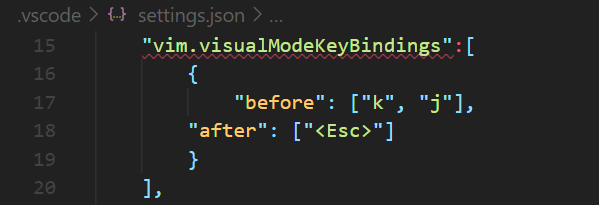
\includegraphics{kj-key.png}

  \begin{quote}
  \begin{itemize}
  \tightlist
  \item
    It is accessible by hitting
    settings\textgreater extensions\textgreater vim\textgreater edit
    keybindings.json {[}blu button{]}
  \item
    I can referens the
  \end{itemize}
  \end{quote}
\item
  and made the settings file with the tab correction:
\end{itemize}
\begin{quote}
\begin{itemize}
\tightlist
\item
  and
  C:\textbackslash Users\textbackslash dashf\textbackslash Desktop\textbackslash VS
  Coding.vscode.vscode\textbackslash settings.json
\end{itemize}
\end{quote}

\#\#\#2\_9: Some navigational shortcuts I practiced some vim commands
navigating words with b,e,w. I also fownd that I can drag a tab in vs
code w my mouse, then I can cycle between the pannels with ctrl+1, or
ctrl+2 or 3

dddd/dddd/I can navigate my tabs in vs code by using my trackpad for
horizontal scroll

\begin{itemize}
\tightlist
\item
  this isnt vs code, but razer, ctrl+caps enter is slow, sliding four
  fingers on the precision trackpad is fast
\end{itemize}

I installed the extension learn vim. I can work thru the lessons by
doing ctrl+shft+p then executing the command learn vim

\#\#\#\#to reopen vscodevim settings: ctrl+shft+p then executing the
command Preferences: Open settings (JSON) or Preferences: Open keyboard

\#\#\#2\_7 I downloaded Code Spell Checker because someone on reddit
said it is accurate, and ignores text that is in camelCase (not
snake\_case)

I learned I can open .ipynb in vs code...

\begin{itemize}
\tightlist
\item
\end{itemize}
# 2021-01-11_1234
#programming
0 update pip to 2.3.\_

VS Code is just a text editor

I installed miniconda and pylance

I can open jypter notebooks, but I lost the introductory screen

\hypertarget{registrars}{%
\subsubsection{Registrars}\label{registrars}}

0 learn from link below how to use registrars to quickly paste text, and
avoid losing anything
[Youtube Vim Registers The Frugal Computer Guy]{https://www.youtube.com/watch?v=yN5L2_f-nUA\&ab_channel=TheFrugalComputerGuy}

[Source Forge Vim Registers]{http://vimdoc.sourceforge.net/htmldoc/change.html\#registers}

[Barbarian Meets Coding Pixel Art Learn Vim how to Copy Paste]{https://www.barbarianmeetscoding.com/boost-your-coding-fu-with-vscode-and-vim/copy-paste/}
# 2021-03-08_1234 Vim Registers
#programming/vim
## Learn Vim
- [x] I am on \#moving fast \#\# move to a specific char. I access the pixel art file with ctrl+shft+p learn vim (or by clicking extensions), then I can work in the text document on the right
Notes from what Ethan showed me 3\_8
\begin{itemize}
\item
  I can access my last 9 things I copied with ditto by pressing
  ctrl+1-9. vim does the same thing in insert mode if I do ctrl+r then
  1-9.
\item
  to save a word in a register

  \begin{enumerate}
  \tightlist
  \item
    In normal mode, I click in a word, then "yank in word"
  \item
    "ayiw

    \begin{itemize}
    \tightlist
    \item
    \item You could add the selected text to the register r by doing "ry. You are copying (yanking) the selected text, and then adding it to the register "r
    \end{itemize}
  \item
    I navigate to where I want to paste (put), then access the Register
  \item
    ctrl+r a
  \end{enumerate}
\item
  0 is a special key that stores the copy clipboard. Every time I copy
  something, it is saved to the clipboard that is specified as the
  destination, and the copy clipboard. When two things are copied, the
  second overwrites the first, but the first is still saved in the copy
  clipboard (I think)
\item
  " is also a special key that stores the system registrar
\end{itemize}

# 2020-10-11_1234
#programming/python
"ctrl+/" Comment out a line that is highlighted with visual-block by pressing "ctrl+/"

I downloaded the most recent windows python, vs code, and vim extension
on my second try I got python to make an appropriate path for vs code (I
also checked with the command prompt)

I watched the yt tutorial below. It sugested downloadin the
don.jayamanne extension pack rather than the sugested

[Chris Hawkes Python for Absolute Beginners]{https://www.youtube.com/watch?v=IZj8hLrkABs\&ab_channel=ChrisHawkes}
(in the python youtube playlist)

x why does this "VS Coding" folder now have a ".json" folder ?where can I
find the Vim shortcuts in the text editor

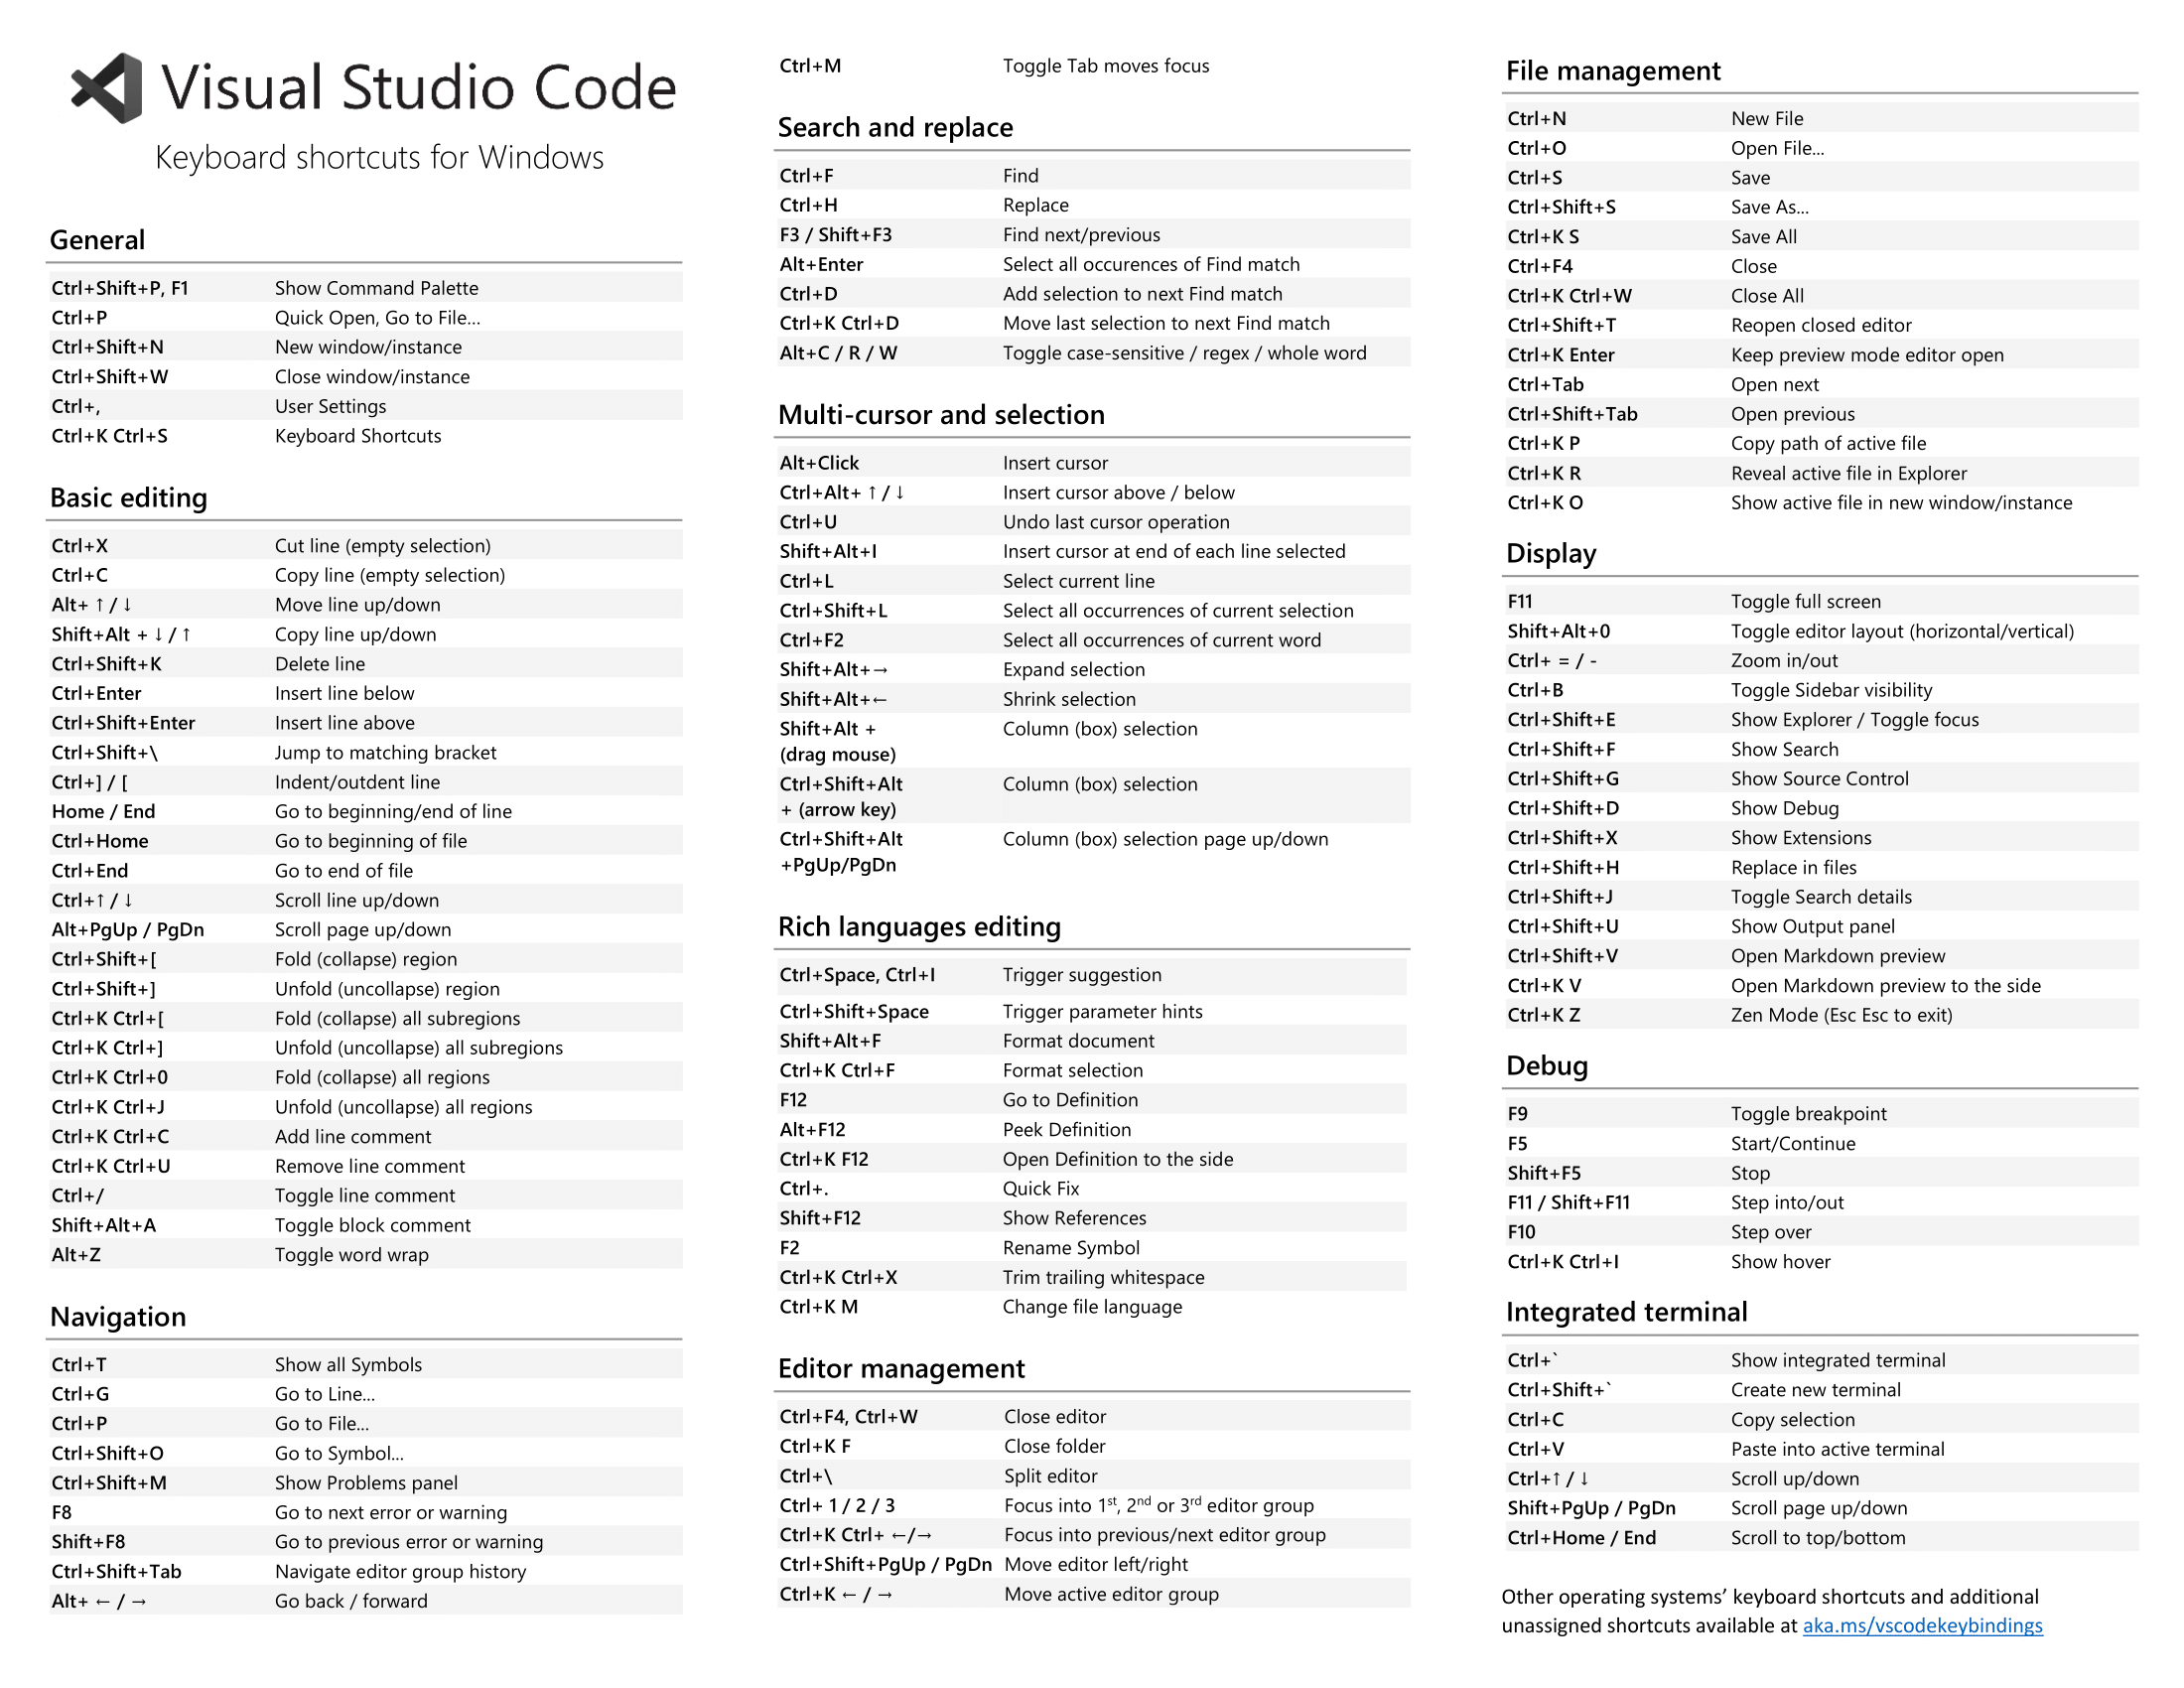
\includegraphics{keyboard-shortcuts-windows (1)-1.png}

